\subsection{Question 1}
\lstinputlisting[caption=Matlab Commands,showstringspaces=false,language=Matlab]{../q1.m}

The code above was run on various incarnations of the matrix \(A\).
For each expirement the matrix \(A\) is 100x100 in dimension.
Each expirement varied the number of intervals the eigenvalues of \(A\) were centered around and how large this interval was.
The number of intervals ranged from 1 to 5.

The conclusion of the expirements was very clear.
The speed of convergence of \(\sigma (S_n)\) towards \(\sigma (A)\) was proportional to the number of intervals the eigenvalues were centered around.
For example, consider the plots below.
This expirement was run with three intervals centered at -3, 4, and 1.
From Figure~\ref{fig:q1_plots}  we see that after three iterations the \(\sigma (S_n)\) is starts to align well with the \(\sigma (A)\) ({\em i.e.,} the three eigenvalues of \(S_n\) align with the three intervals).
This is true in general.
Specifically the convergence happens at a rate of \(\frac{1}{|I|}\) where \(|I|\) is the number of intervals the eigenvalues of \(A\) are centered around.

\newpage
\lstinputlisting[caption=Matlab Commands,showstringspaces=false,language=Matlab]{../my_gmres.m}

\begin{figure}[t]
  \centering
  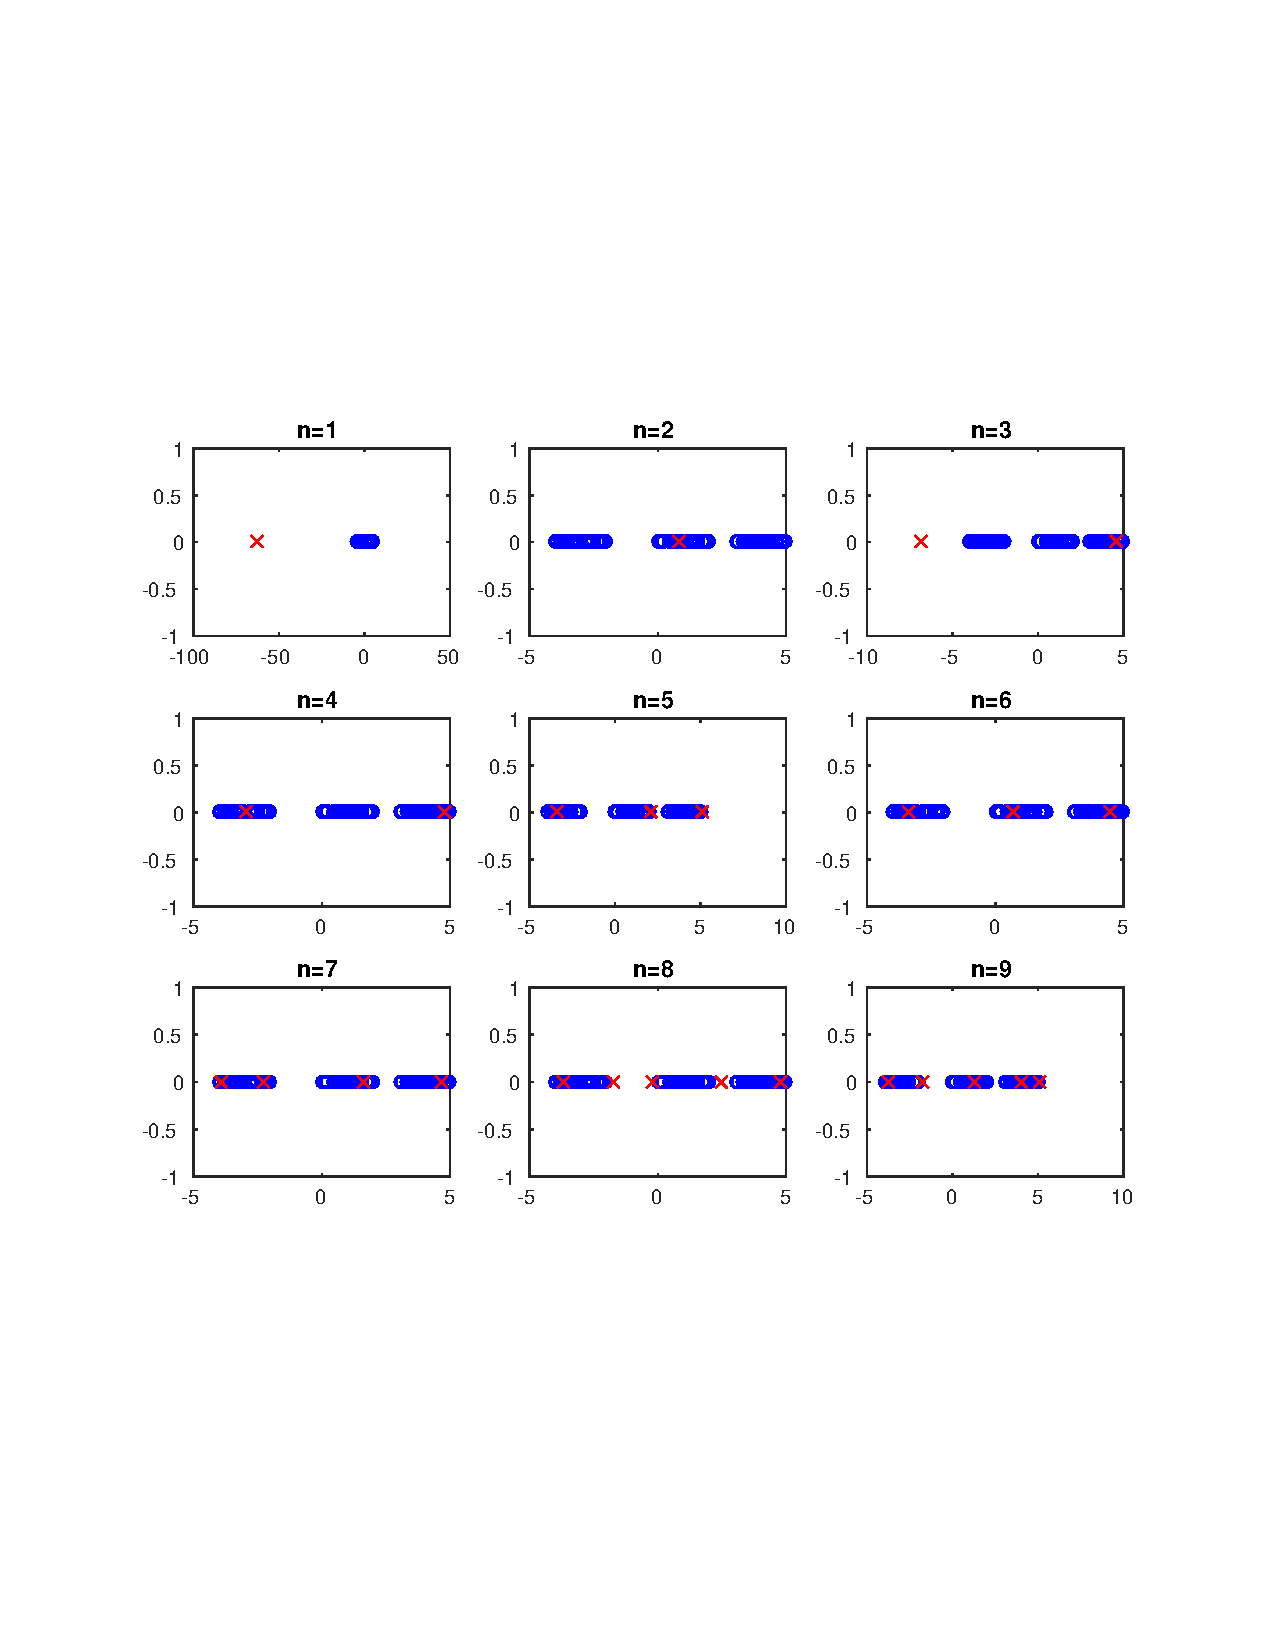
\includegraphics[trim=10mm 70mm 10mm 70mm, width=1.0\textwidth]{../q1_plots}
  \caption{Plots of \(\sigma (S_n)\) (red) and  \(\sigma (A)\) (blue). Plots correspond to stopping GMRES after \(n\) iterations.}
  \label{fig:q1_plots}
\end{figure}

\newpage
\subsection{Question 2}

\lstinputlisting[caption=Matlab Commands,showstringspaces=false,language=Matlab]{../q2_all}

\newpage
\lstinputlisting[caption=Matlab Commands,showstringspaces=false,language=Matlab]{../q2.m}

As with the expirement from Question 1 the number of intervals was kept constant at 3 and the interval ranges were varied from 0.5 to 2.
The results obtained reflect the sentiments expressed above.
The convergence (relative error decreased) of \(\sigma (S_n)\) to \(\sigma (A)\) occurred at a rate of \(\frac{1}{|I|}\).
Therefore after ten iterations the error was extremely small (0.000154) and became almost negligible after that.
After ninety iterations the \(\sigma (S_n)\) was essentially the same as the \(\sigma (A)\) and after one hundred there was complete convergence.
However, it makes little sense to iterate this long as the cost trade off of using an indirect method is lost ({\em i.e.,} the complexity is \(O(m^3)\).
Figure~\ref{fig:q2_plots} demonstrates the reduction in error at the different values of \(n\).

\begin{figure}[th]
  \centering
  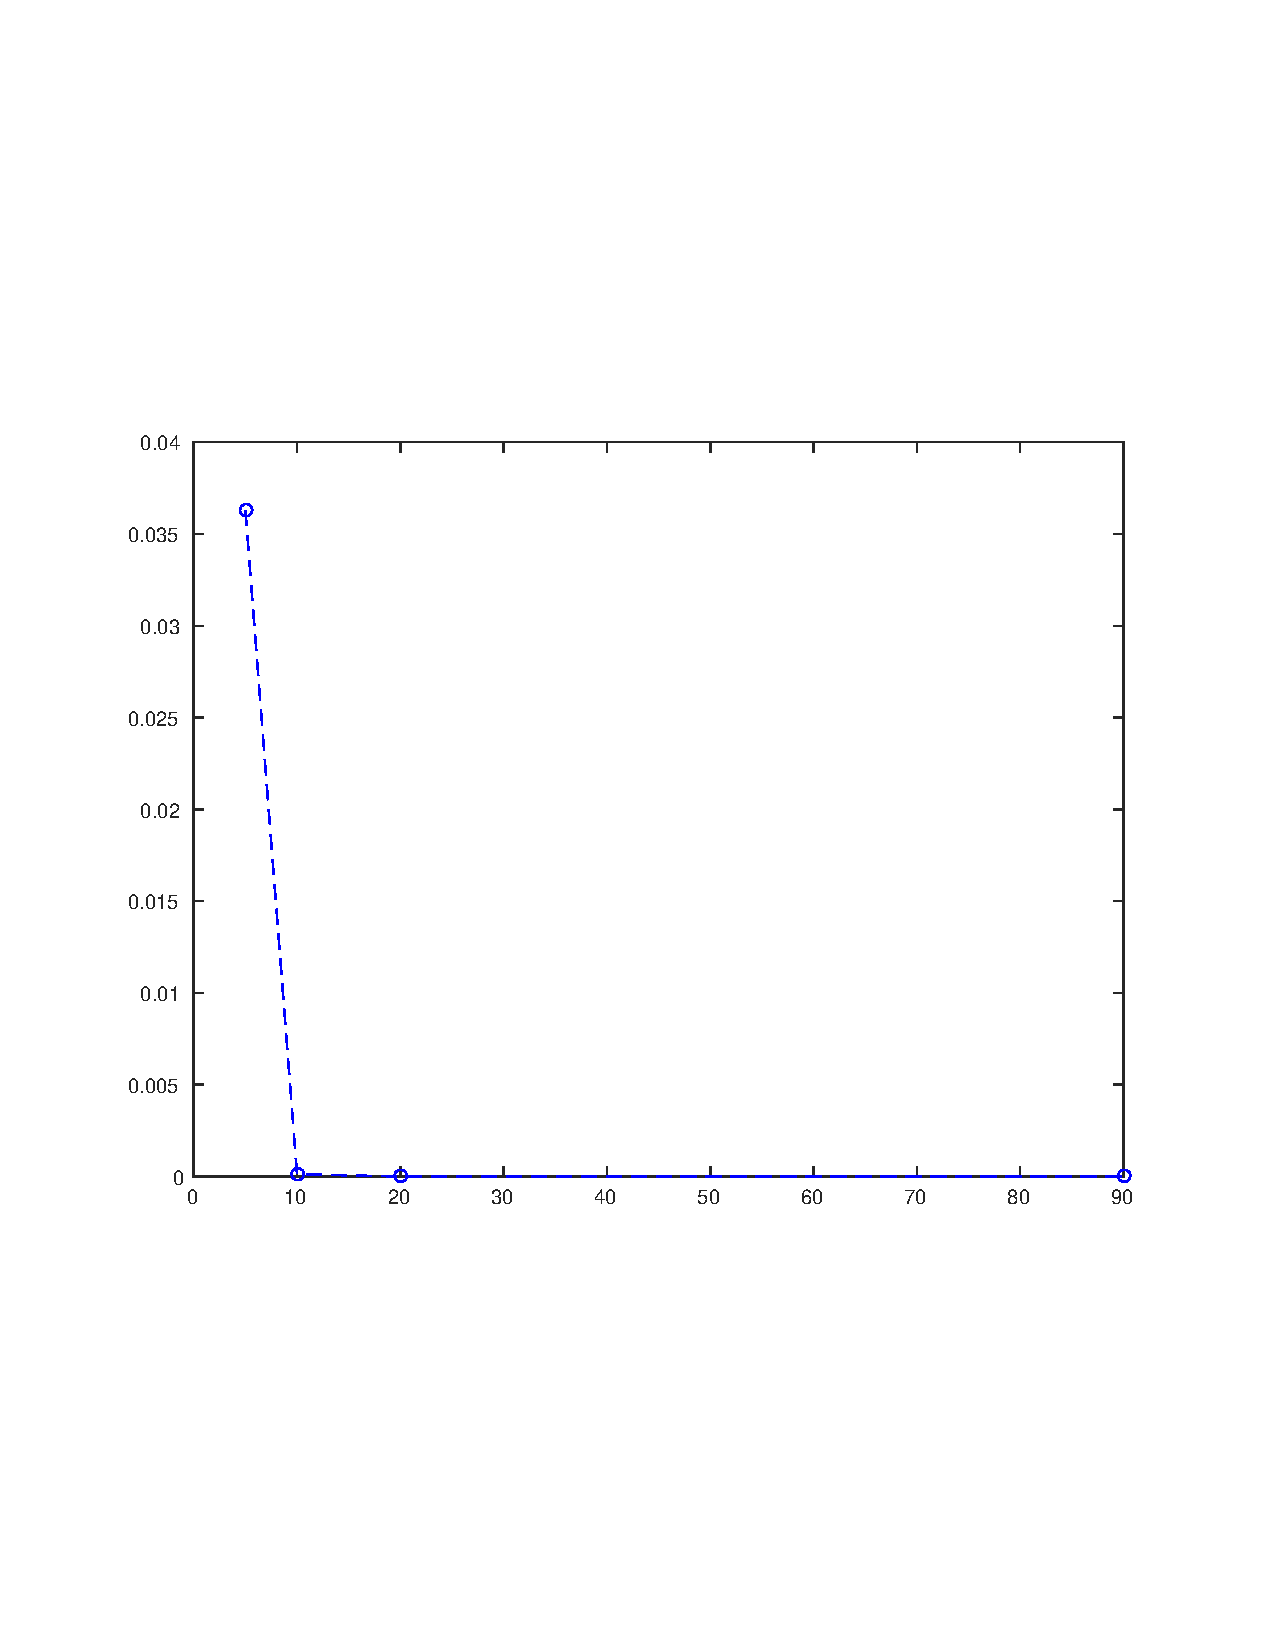
\includegraphics[trim=10mm 70mm 10mm 70mm, width=1.0\textwidth]{../q2_plots}
  \caption{Plot showing the relative error \(||A\tilde{x}-b||_2\) for different values of \(n\).}
  \label{fig:q2_plots}
\end{figure}

\newpage
\subsection{Question 3}

\lstinputlisting[caption=Matlab Commands,showstringspaces=false,language=Matlab]{../q3.m}

\newpage
The experiment setup was similar to the two expirements above, except the value of \(k\) was the variable in this case.
Figure~\ref{fig:q3_plots} shows one of these expirements.
It is clear from Figure~\ref{fig:q3_plots} that the first two singular values of \(A\) are much larger than the other singular values of \(A\).
Specifically, the first two singular values are roughly \(k*10\) times and \(k\) times larger than the other singular values.
This makes intuitive sense as \(A\) is built out of an underlying matrix where the first two rows are \(k\) times larger than the other rows.
Therefore, the first two singular values and left singular vectors of \(A\) capture the structure of \(A\) quite well.

\begin{figure}[t]
  \centering
  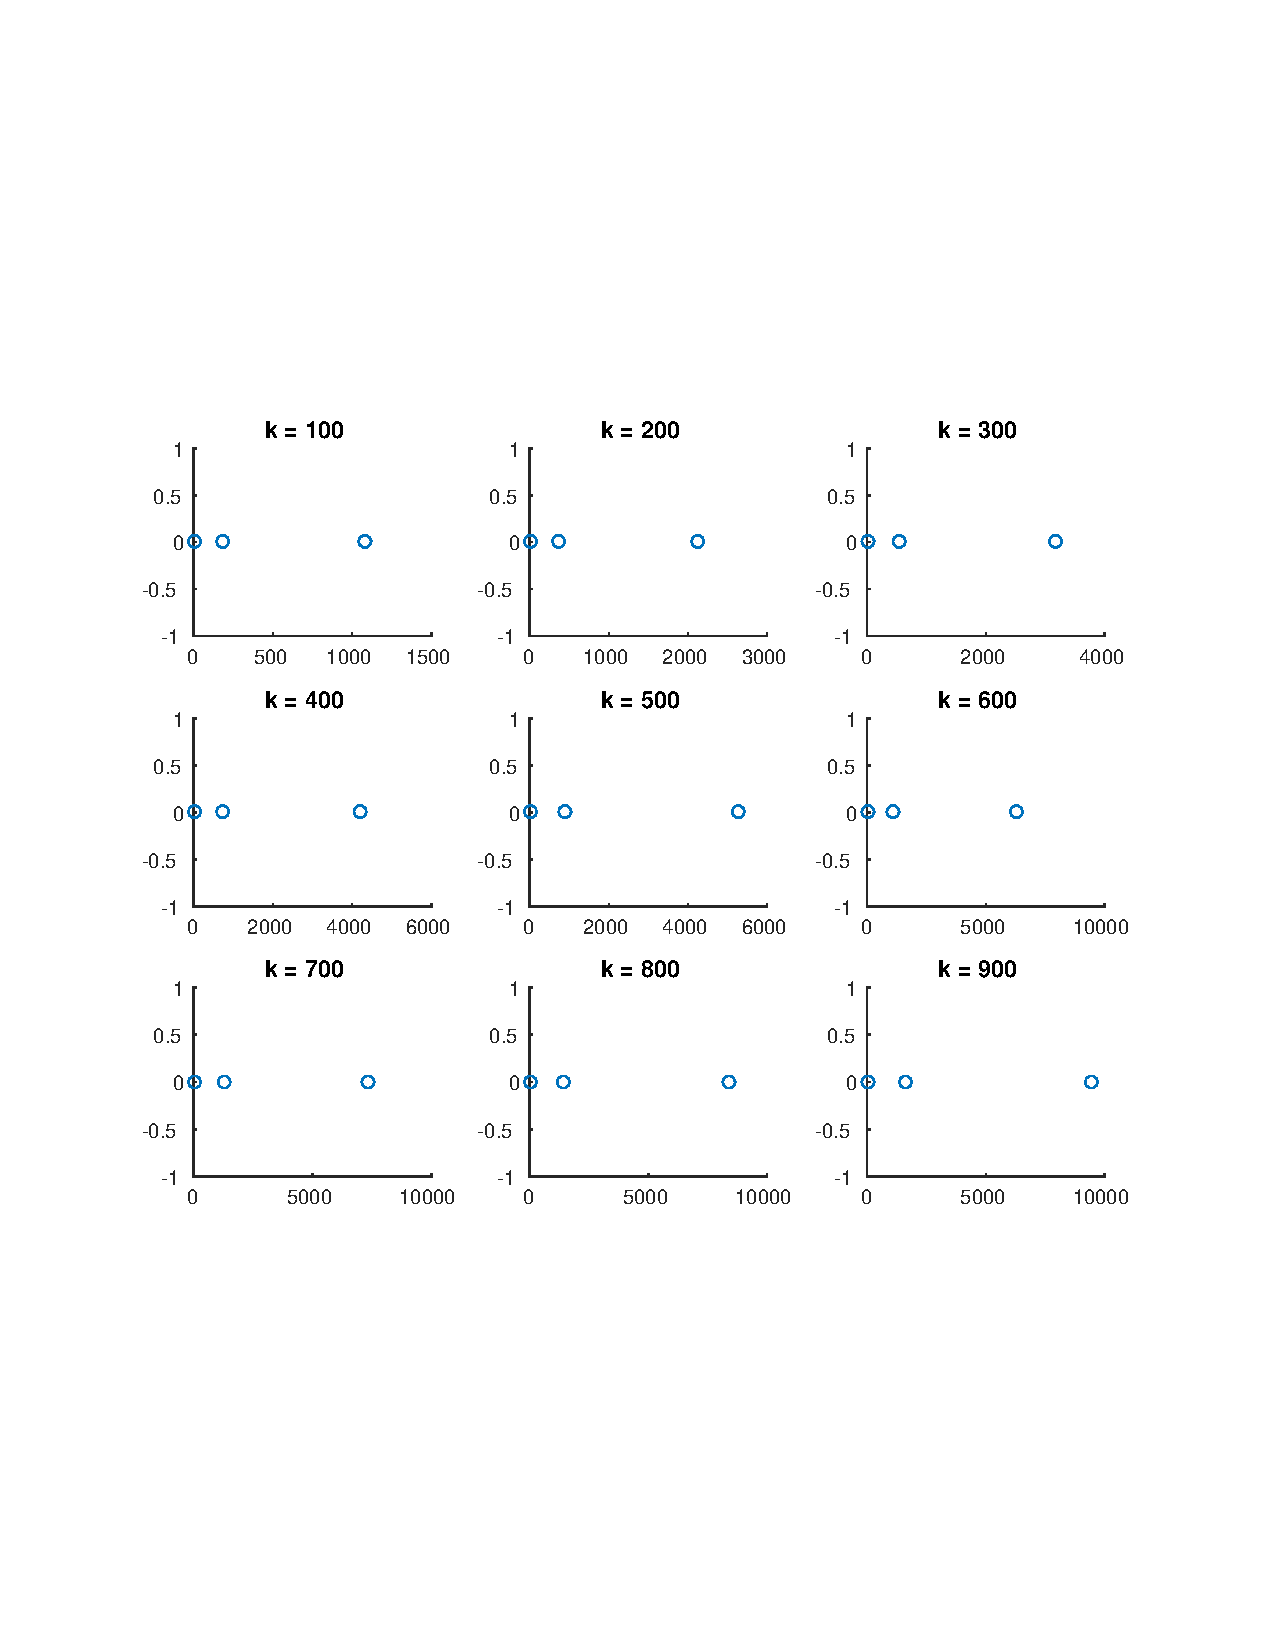
\includegraphics[trim=10mm 70mm 10mm 70mm, width=1.0\textwidth]{../q3_plots}
  \caption{Plots of singular values of \(A\) at various \(k\). Note, the first two singular values are much larger than the rest (~\(k*10\) and \(k\) times larger respectively).}
  \label{fig:q3_plots}
\end{figure}

\newpage
\lstinputlisting[caption=Matlab Commands,showstringspaces=false,language=Matlab]{../generate_interval_matrix.m}

%\lstinputlisting[caption=Matlab Commands,showstringspaces=false,language=Matlab]{../lu_sym.m}
%\begin{figure}[th]
%  \centering
%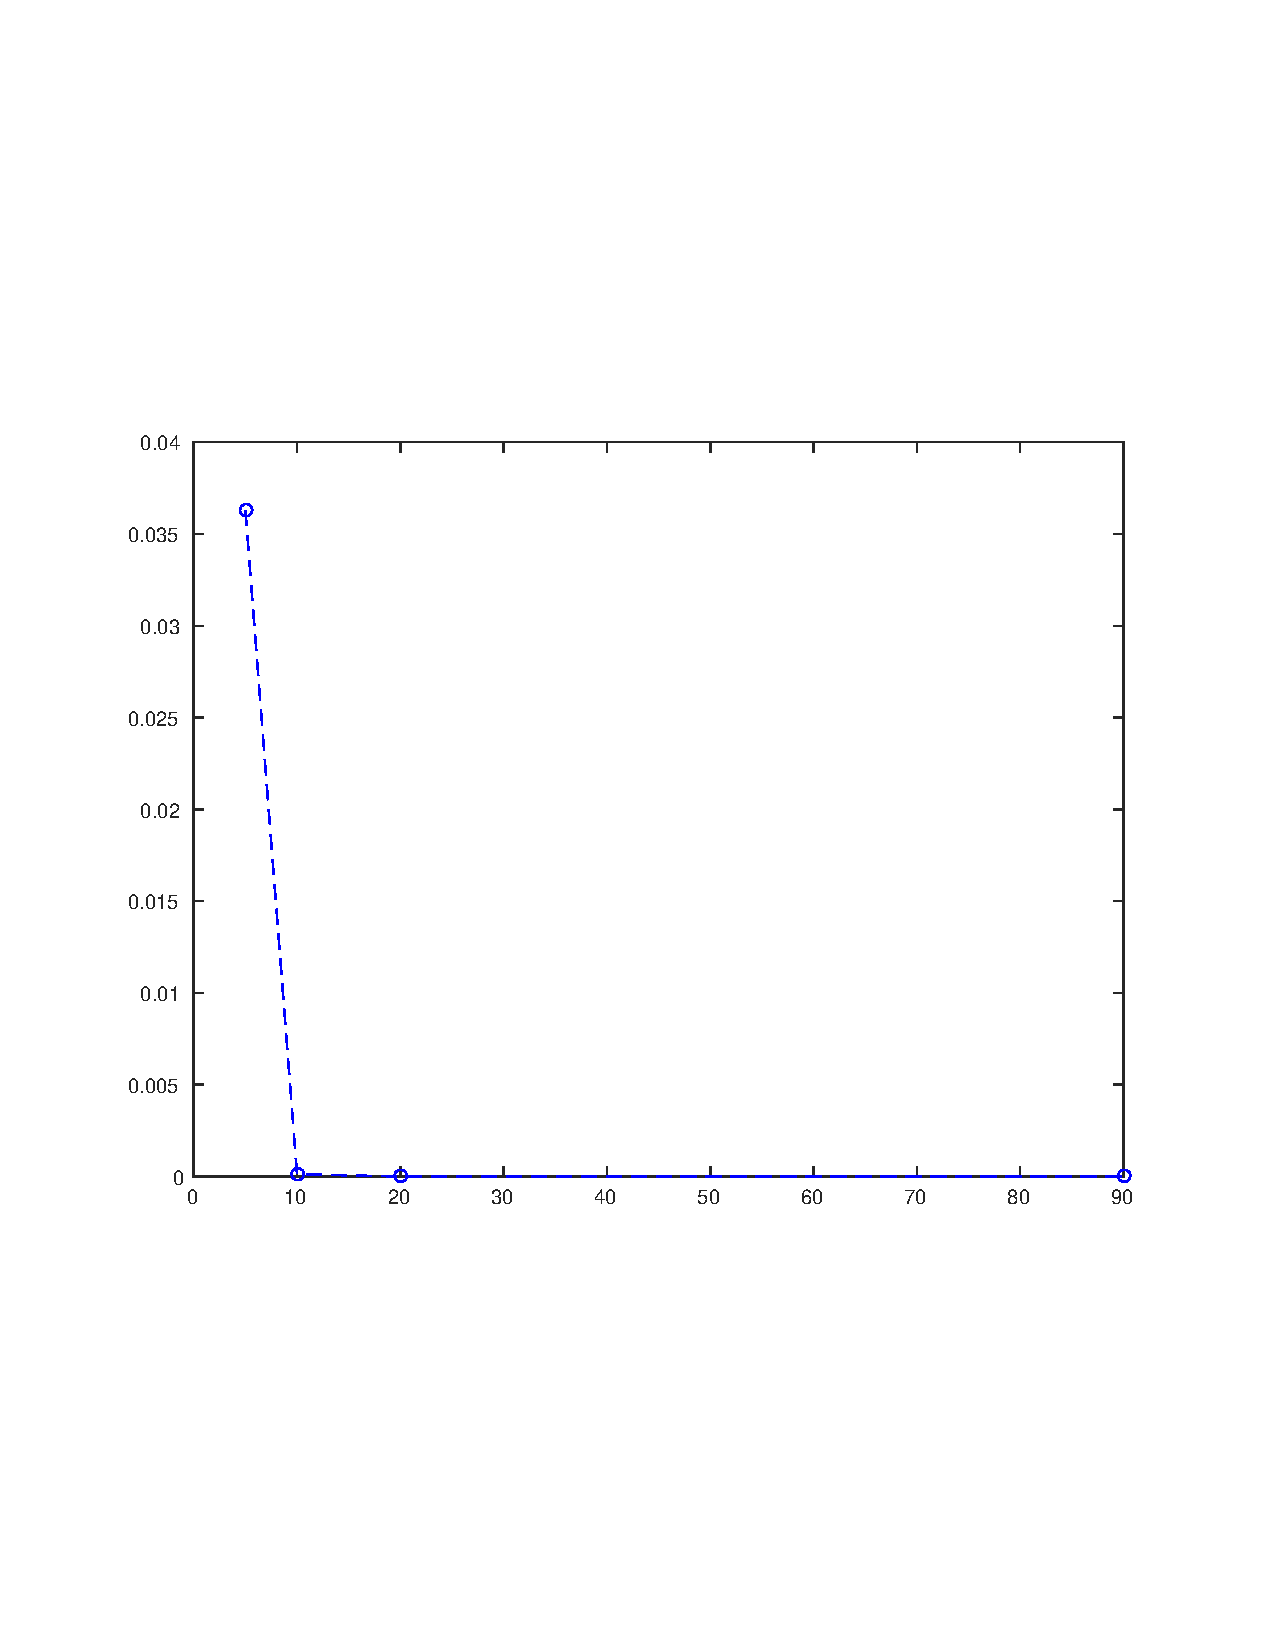
\includegraphics[trim=10mm 70mm 10mm 70mm, width=1.0\textwidth]{../q2_plots}
%\end{figure}
